
上一节的末尾,我们找出了程序在什么地方花费了大部分的执行时间。在使用“明显的”和“简单的”优化后,出现了事与愿违的情况,使程序运行速度变慢,我们也感到惊讶。现在很清楚,我们必须更详细地研究性能关键函数。

We already have the tools for that: the overall program is exercising this code, and we have ways to measure its performance. But we're not really interested in the rest of the program anymore, at least not until we solve the performance issues we already identified. 

Working with a large program to optimize just a few lines of code has the following two major drawbacks:

First of all, even though the few lines are identified as performance-critical, it doesn't mean the rest of the program takes no time at all (in our demo example, it does, but recall that this example is supposed to represent the entire large program you're working on). You may be waiting for hours before the large program gets to the interesting point, either because the entire job is that long or because the performance-critical function is called only under certain conditions, like a particular request coming over the net.

Second, working with a large program just takes more time: the compile and link times are longer, your work may be interacting with code changes made by other programmers, even editing takes longer because all the extra code is distracting. The bottom line, at this point, is we are interested in just one function, so we would like to be able to call this function and measure the results. This is where micro-benchmarking comes in.

\subsubsubsection{2.5.1\hspace{0.2cm}Basics of micro-benchmarking}

In a nutshell, micro-benchmarking is just a way to do what we just said we want to do: run a small chunk of code and measure its performance. In our case, it's just one function, but it could be a more complex code fragment, too. What's important is that this code fragment could be invoked easily with the right starting conditions: for a function, it's just the arguments, but for a larger fragment, a more complex internal state may have to be recreated.

In our case, we know exactly what arguments we need to call the string comparison function with – we constructed the arguments ourselves. The second thing we need is to measure the execution time; we have already seen the timers that can be used for this purpose. With this in mind, we can write a very simple benchmark that calls several variants of our string comparison function and reports the results:

\begin{lstlisting}[style=styleCXX]
bool compare1(const char* s1, const char* s2) {
	int i1 = 0, i2 = 0;
	char c1, c2;
	while (1) {
		c1 = s1[i1]; c2 = s2[i2];
		if (c1 != c2) return c1 > c2;
		++i1; ++i2;
	}
}
bool compare2(const char* s1, const char* s2) {
	unsigned int i1 = 0, i2 = 0;
	char c1, c2;
	while (1) {
		c1 = s1[i1]; c2 = s2[i2];
		if (c1 != c2) return c1 > c2;
		++i1; ++i2;
	}
}
int main() {
	constexpr unsigned int N = 1 << 20;
	unique_ptr<char[]> s(new char[2*N]);
	::memset(s.get(), 'a', 2*N*sizeof(char));
	s[2*N-1] = 0;
	system_clock::time_point t0 = system_clock::now();
	compare1(s.get(), s.get() + N);
	system_clock::time_point t1 = system_clock::now();
	compare2(s.get(), s.get() + N);
	system_clock::time_point t2 = system_clock::now();
	cout << duration_cast<microseconds>(t1 - t0).count() <<
	  "us " << duration_cast<microseconds>(t2 - t1).count() <<
	  "us" << endl;
}
\end{lstlisting}

In this program, we test only two of the comparison functions, both without the end of loop condition, one with an int index and the other with an unsigned int index. Also, we will not be repeating the \#include and using statements in the subsequent listings. The input data is just a long string filled with the same character from start to end, so the substring comparison will run all the way to the end of the string. We can, of course, benchmark on any data we need, but let's start with the simplest case.

The program looks like it will do exactly what we need… at least until we run it:

%\hspace*{\fill} \\ %插入空行
\begin{center}
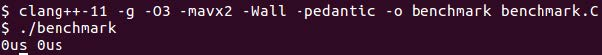
\includegraphics[width=0.9\textwidth]{content/1/chapter2/images/22.jpg}\\
图 2.22
\end{center}

Zero time, either way. What went wrong? Perhaps, the execution time for a single function call is simply too fast to be measured? This is not a bad guess, and we can address this problem easily: if one call is too short, we just need to make more calls:

\begin{lstlisting}[style=styleCXX]
int main() {
	constexpr unsigned int N = 1 << 20;
	constexpr int NI = 1 << 11;
	unique_ptr<char[]> s(new char[2*N]);
	::memset(s.get(), 'a', 2*N*sizeof(char));
	s[2*N-1] = 0;
	system_clock::time_point t0 = system_clock::now();
	for (int i = 0; i < NI; ++i) {
		compare1(s.get(), s.get() + N);
	}
	system_clock::time_point t1 = system_clock::now();
	for (int i = 0; i < NI; ++i) {
		compare2(s.get(), s.get() + N);
	}
	system_clock::time_point t2 = system_clock::now();
	cout << duration_cast<microseconds>(t1 - t0).count() <<
	  "us " << duration_cast<microseconds>(t2 - t1).count() <<
	  "us" << endl;
}
\end{lstlisting}

We can increase the number of iterations NI until we get some results, right? Not so fast:

%\hspace*{\fill} \\ %插入空行
\begin{center}
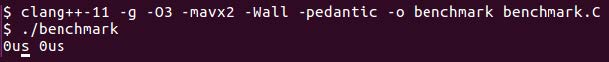
\includegraphics[width=0.9\textwidth]{content/1/chapter2/images/23.jpg}\\
图 2.23
\end{center}

Too fast, actually, but why? Let us step through the program in the debugger and see what it actually did:

%\hspace*{\fill} \\ %插入空行
\begin{center}
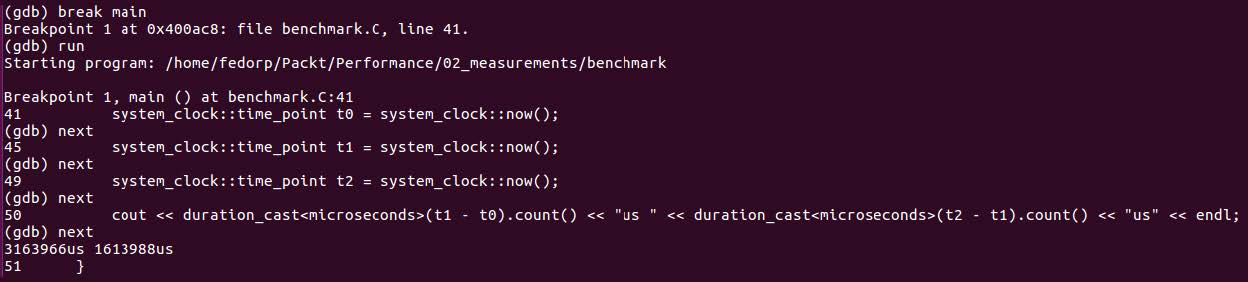
\includegraphics[width=0.9\textwidth]{content/1/chapter2/images/24.jpg}\\
图 2.24
\end{center}

We set the breakpoint in main, so the program is paused as soon as it launches, then we execute the program line by line… except, that's not all the lines we have written! Where is the rest of the code? We can guess that the compiler is to blame, but why? We need to learn more about compiler optimizations.

\subsubsubsection{2.5.2\hspace{0.2cm}Micro-benchmarking and compiler optimizations}

To understand this mystery of the missing code, we have to take a fresh look at what the missing code actually does. It creates some strings, calls the comparison functions, and … there is no "and." Nothing else happens. Other than watching the code scroll by in the debugger, how would you know, just by running this program, if this code was executed? You cannot. The compiler has arrived at the same conclusion, way ahead of us. Since the programmer cannot tell the difference between executing and not executing a part of the code, the compiler has optimized it out. But wait, you say, the programmer can tell the difference: it takes much less time to do nothing than to do something. And here we come to a very important concept from the C++ standard that is critical to the understanding of compiler optimizations: the observable behavior.

The standard says that the compiler can make whatever changes it wants to the program as long as the effect of these changes does not alter the observable behavior. The standard is also very specific about what constitutes the observable behavior:

\begin{enumerate}
\item Accesses (reads and writes) to volatile objects occur strictly according to the semantics of the expressions in which they occur. In particular, they are not reordered with respect to other volatile accesses on the same thread.
\item At program termination, data written to files is exactly as if the program was executed as written.
\item Prompting text that is sent to interactive devices will be shown before the program waits for input. More generally, input and output operations cannot be omitted or rearranged.
\end{enumerate}

There are a few exceptions to the preceding rules, none of which apply to our program. The compiler must follow the as-if rule: the optimized program should show the same observable behavior as if it was executed exactly as written, line for line. Now note what is not included in the preceding list: running the program under debugger does not constitute observable behavior. Neither does execution time, otherwise, no program could be optimized to make it faster.

With this new understanding, let us take another look at the benchmark code: the results of the string comparison do not affect the observable behavior in any way, so the entire computation can be done or omitted at the compiler's discretion. This observation also gives us a way to fix this problem: we have to make sure that the result of the computation affects the observable behavior. One way to do it is to take advantage of the volatile semantics described previously:

\hspace*{\fill} \\ %插入空行
\noindent
\textbf{05\_compare\_timer.C}
\begin{lstlisting}[style=styleCXX]
int main() {
	constexpr unsigned int N = 1 << 20;
	constexpr int NI = 1 << 11;
	unique_ptr<char[]> s(new char[2*N]);
	::memset(s.get(), 'a', 2*N*sizeof(char));
	s[2*N-1] = 0;
	volatile bool sink;
	system_clock::time_point t0 = system_clock::now();
	for (int i = 0; i < NI; ++i) {
		sink = compare1(s.get(), s.get() + N);
	}
	system_clock::time_point t1 = system_clock::now();
	for (int i = 0; i < NI; ++i) {
		sink = compare2(s.get(), s.get() + N);
	}
	system_clock::time_point t2 = system_clock::now();
	cout << duration_cast<microseconds>(t1 - t0).count() <<
	  "us " << duration_cast<microseconds>(t2 - t1).count() <<
	  "us" << endl;
}
\end{lstlisting}

Now the result of every call to the comparison functions is written into a volatile variable, and, according to the standard, these values must be correct and written in the right order. The compiler now has no choice but to call our comparison functions and get the results. The way these results are computed can still be optimized as long as the result itself does not change. This is exactly what we want: we want the compiler to generate the best code for the comparison functions, hopefully, the same code it generates in the real program. We just don't want it to drop these functions altogether. Running this benchmark shows that we have finally achieved our goal, the code is definitely running:

%\hspace*{\fill} \\ %插入空行
\begin{center}
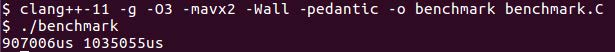
\includegraphics[width=0.9\textwidth]{content/1/chapter2/images/25.jpg}\\
图 2.25
\end{center}

The first value is the runtime of the compare1() function, which uses int indices, and it is indeed slightly faster than the unsigned int version (but don't put too much faith into these results just yet).

The second option for entangling our computations with some observable behavior is to simply print out the results. However, this can get a bit tricky. Consider the straightforward attempt:

\begin{lstlisting}[style=styleCXX]
int main() {
	constexpr unsigned int N = 1 << 20;
	constexpr int NI = 1 << 11;
	unique_ptr<char[]> s(new char[2*N]);
	::memset(s.get(), 'a', 2*N*sizeof(char));
	s[2*N-1] = 0;
	bool sink;
	system_clock::time_point t0 = system_clock::now();
	for (int i = 0; i < NI; ++i) {
		sink = compare1(s.get(), s.get() + N);
	}
	system_clock::time_point t1 = system_clock::now();
	for (int i = 0; i < NI; ++i) {
		sink = compare2(s.get(), s.get() + N);
	}
	system_clock::time_point t2 = system_clock::now();
	cout << duration_cast<microseconds>(t1 - t0).count() <<
	  "us " << duration_cast<microseconds>(t2 - t1).count() <<
	  "us" << sink << endl;
}
\end{lstlisting}

Note that the variable sink is no longer volatile, but instead, we write out its final value. This does not work as well as you might expect:

%\hspace*{\fill} \\ %插入空行
\begin{center}
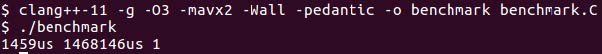
\includegraphics[width=0.9\textwidth]{content/1/chapter2/images/26.jpg}\\
图 2.26
\end{center}

The execution time of the function compare2() is in the same ballpark as before, but compare1() appears to be much faster now. Of course, by now, we know enough to understand that this "improvement" is illusory: the compiler simply figured out that the result of the first call is overwritten by the second call and, therefore, does not affect the observable behavior.

This brings up an interesting question: why didn't the compiler figure out that the second iteration of the loop gives the same result as the first one and optimized away every call to the comparison functions except the first one, for each function? It could have, if the optimizer were advanced enough, and then we would have to do more to get around it: generally, compiling the functions as separate compilation units is enough to prevent any such optimizations, although some compilers are capable of whole-program optimizations, so you may have to turn them off when running micro-benchmarks.

Note also that our two benchmark runs have produced somewhat different values even for the execution time of the function that wasn't optimized away. If you run the program again, you will get yet another value, also somewhere in the same range, but slightly different. This isn't good enough: we need more than just ballpark figures. We could run the benchmark several times, figure out how many repetitions we need, and compute the average time, but we don't have to do it manually. We don't have to write code to do this either, because such code has already been written and is available as one of several microbenchmarking tools. We are going to learn about one such tool now.

\subsubsubsection{2.5.3\hspace{0.2cm}Google Benchmark}

Writing a micro-benchmark involves a lot of boilerplate code, mostly for measuring time and accumulating results. Furthermore, this code is critical for the accuracy of the measurements. There are several good-quality micro-benchmark libraries available. In this book, we use the Google Benchmark library. The instructions for downloading and installing the library can be found in the Technical requirements section. In this section, we will describe how to use the library and interpret the results.

To use the Google Benchmark library, we have to write a small program that will prepare the inputs and execute the code we want to benchmark. This is a basic Google Benchmark program for measuring the performance of one of our string comparison functions:

\hspace*{\fill} \\ %插入空行
\noindent
\textbf{10\_compare\_mbm.C}
\begin{lstlisting}[style=styleCXX]
#include "benchmark/benchmark.h"
using std::unique_ptr;
bool compare_int(const char* s1, const char* s2) {
	char c1, c2;
	for (int i1 = 0, i2 = 0; ; ++i1, ++i2) {
		c1 = s1[i1]; c2 = s2[i2];
		if (c1 != c2) return c1 > c2;
	}
}
void BM_loop_int(benchmark::State& state) {
	const unsigned int N = state.range(0);
	unique_ptr<char[]> s(new char[2*N]);
	::memset(s.get(), 'a', 2*N*sizeof(char));
	s[2*N-1] = 0;
	const char* s1 = s.get(), *s2 = s1 + N;
	for (auto _ : state) {
		benchmark::DoNotOptimize(compare_int(s1, s2));
	}
	state.SetItemsProcessed(N*state.iterations());
}
BENCHMARK(BM_loop_int)->Arg(1<<20);
BENCHMARK_MAIN();
\end{lstlisting}

Every Google benchmark program must include the header for the library, benchmark/benchmark.h, plus, of course, any other headers needed to compile the code we want to measure (they are omitted in the preceding listing). The program itself consists of a number of benchmark "fixtures," each one is just a function with a specific signature: it takes one parameter, benchmark::State, by reference, and returns nothing. The parameter is an object provided by the Google Benchmark library to interface with the library itself. 

We need one fixture for each code fragment, such as a function that we want to benchmark. The first thing we do in each benchmark fixture is to set up the data we need to use as inputs for the code we want to run. More generally, we can say that we need to recreate the initial state of this code to represent what it would be in the real program. In our case, the input is the string, so we need to allocate and initialize the string. We can hardcode the size of the string into the benchmark, but there is also a way to pass arguments into a benchmark fixture. Our fixture uses one argument, the string length, which is an integer accessed as state.range(0). It is possible to pass arguments of other types, please refer to the documentation of the Google Benchmark library for details.

The entire setup is free in the sense of the benchmark measurements: we do not measure the time it takes to prepare the data. The code whose execution time is measured goes into the body of the benchmarking loop, for (auto \_ : state) { … }. In the older examples, you can find this loop written as while (state.KeepRunning()) { … }, which does the same thing but slightly less efficiently. The library measures the time it takes to do each iteration and decides how many iterations it wants to do to accumulate enough measurements to reduce the random noise that is inevitable in measuring the run time of a small fragment of code. Only the run time of the code inside the benchmarking loop is measured.

The loop exits when the measurement is accurate enough (or a certain time limit is reached). After the loop, we usually have some code to clean up the data that was initialized earlier, although in our case, this cleanup is handled by the destructor of the std::unique\_ptr object. We can also make calls on the state object to affect what results are reported by the benchmark. The library always reports the average time it takes to run one iteration of the loop, but sometimes it is more convenient to express the program speed in some other way. For our string comparison, one option is to report the number of characters per second processed by the code. We can do it by calling state. SetItemsProcessed() with the number of characters we processed during the entire run, N characters per iteration (or 2*N if you want to count both substrings; items can count whatever you define as a unit of processing).

Nothing is going to happen just because we defined a benchmark fixture, we need to register it with the library. This is done using the BENCHMARK macro; the argument of the macro is the name of the function. By the way, there is nothing special about that name, it can be any valid C++ identifier; that ours begins with BM\_ is merely a naming convention we follow in this book. The BENCHMARK macro is also where you will specify any arguments you want to pass to the benchmark fixture. The arguments and other options affecting the benchmark are passed using the overloaded arrow operator, for example:

\begin{lstlisting}[style=styleCXX]
BENCHMARK(BM_loop_int)->Arg(1<<20);
\end{lstlisting}

This line registers the benchmark fixture BM\_loop\_int with one argument, 1<<20, that can be retrieved inside the fixture by calling state.range(0). We will see more examples of different arguments throughout this book, and even more can be found in the library documentation.

You will also notice that there is no main() in the preceding code listing; instead, there is another macro, BENCHMARK\_MAIN(). The main() is not written by us but provided by the Google Benchmark library, and it does all the necessary work of setting up the benchmarking environment, registering the benchmarks, and executing them.

Let us return for a moment to the code we want to measure and examine it more closely:

\begin{lstlisting}[style=styleCXX]
for (auto _ : state) {
	benchmark::DoNotOptimize(compare_int(s1, s2));
}
\end{lstlisting}

The benchmark::DoNotOptimize(…) wrapper function plays a role similar to the volatile sink we have used before: it ensures that the compiler does not optimize away the entire call to compare\_int(). Note that it does not actually turn off any optimizations; in particular, the code inside the parentheses is optimized as usual, which is what we want. All it does is tells the compiler that the result of the expression, in our case, the return value of the comparison function, should be considered "used" as if it was printed out and cannot be simply discarded.

We are now ready to compile and run our first micro-benchmark:

%\hspace*{\fill} \\ %插入空行
\begin{center}
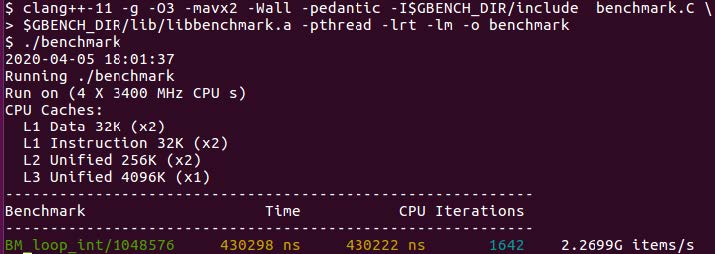
\includegraphics[width=0.9\textwidth]{content/1/chapter2/images/27.jpg}\\
图 2.27
\end{center}

The compile line now has to list the path to the Google Benchmark include files and the library; several additional libraries are needed by the Google Benchmark library libbenchmark.a. Once invoked, the benchmark program prints some information about the system we are running on, then it executes every fixture that was registered, with all their arguments. We get one line of output for every benchmark fixture and a set of arguments; the report includes the average real time and the average CPU time of a single execution of the body of the benchmark loop, how many times the loop was executed, and any other statistics we have attached to the report (in our case, the number of characters per second processed by the comparison, over 2G characters per second). How much do these numbers vary from run to run? The benchmark library can calculate that for us if we enable the statistics collection with the right command-line arguments.

For example, to repeat the benchmark ten times and report the results, we would run the benchmark like so:

%\hspace*{\fill} \\ %插入空行
\begin{center}
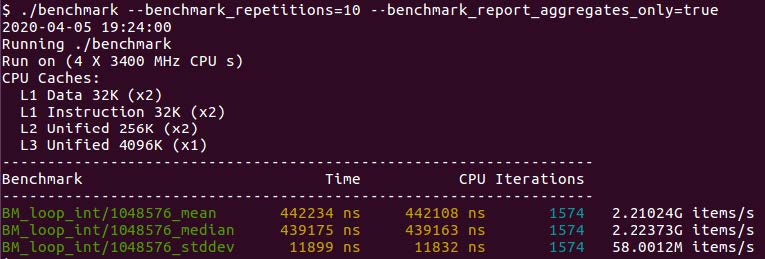
\includegraphics[width=0.9\textwidth]{content/1/chapter2/images/28.jpg}\\
图 2.28
\end{center}

It looks like the measurements are pretty accurate; the standard deviation is quite small. Now we can benchmark the different variants of the substring comparison function against each other and figure out which one is the fastest. But before we do that, I have to let you in on a big secret.

\subsubsubsection{2.5.4\hspace{0.2cm}Micro-benchmarks are lies}

You will discover it soon enough as you start running more and more micro-benchmarks. At first, the results make sense, you're making good optimizations, and everything looks great. Then you make some small change and get a very different result. You go back to investigate, and now the same tests you already ran give very different numbers. Eventually, you come up with two almost identical tests that show completely opposite results, and you realize that you just can't trust micro-benchmarks. It will destroy your faith in micro-benchmarks, and the only thing I can do about it is to destroy it now, in a controlled manner, while we can still salvage something from the wreckage.

The fundamental problem with micro-benchmarks and any other detailed performance measurements is that they strongly depend on the context. As you read through the rest of the book, you will understand more and more that the performance behavior of modern computers is very complex. The results do not just depend on what the code is doing, but also on what the rest of the system is doing at the same time, on what it was doing earlier, and on the path the execution took through the code before it got to the point of interest. None of these things are replicated in a micro-benchmark.

Instead, the benchmark has its own context. The authors of the benchmarking libraries are not ignorant of this problem, and they try to counter it the best they can. For example, unseen to you, the Google Benchmark library does a burn-in on every test: the first few iterations may have very different performance characteristics from the rest of the run, so the library ignores the initial measurements until the results "settle." But this also defines a particular context, probably different from the real program where every call to the function is repeated only once (on the other hand, sometimes we do end up calling the same function with the same arguments many times throughout the run of the program, so that could be a different context).

There is nothing you can do to faithfully reproduce the real environment of a large program in every detail before running the benchmark. But some details are more important than others. In particular, the greatest source of contextual differences, by far, is the compiler, or, more specifically, the optimizations it does on a real program versus the micro-benchmark. We have already seen how the compiler stubbornly tries to figure out that the entire micro-benchmark is basically a very slow way of doing nothing useful (or at least nothing observable), and replace it with a much faster way of doing the same. The DoNotOptimize wrapper we used earlier gets us around some of the problems caused by the compiler optimizations.

However, there is still the possibility that the compiler may, for example, figure out that every call to the function returns the same result. Also, because the function definition is in the same file as the call site, the compiler can inline the entire function and use any information it can gather about the arguments to optimize the function code. Such optimizations would not be available in the general case when the function is called from another compilation unit. 

To represent the real situation more accurately in our micro-benchmark, we can move the comparison function into its own file and compile it separately. Now we have one file (compilation unit) with just the benchmark fixtures:

\hspace*{\fill} \\ %插入空行
\noindent
\textbf{11\_compare\_mbm.C}
\begin{lstlisting}[style=styleCXX]
#include "benchmark/benchmark.h"
extern bool compare_int(const char* s1, const char* s2);
extern bool compare_uint(const char* s1, const char* s2);
extern bool compare_uint_l(const char* s1, const char* s2,
unsigned int l);
void BM_loop_int(benchmark::State& state) {
	const unsigned int N = state.range(0);
	unique_ptr<char[]> s(new char[2*N]);
	::memset(s.get(), 'a', 2*N*sizeof(char));
	s[2*N-1] = 0;
	const char* s1 = s.get(), *s2 = s1 + N;
	for (auto _ : state) {
		benchmark::DoNotOptimize(compare_int(s1, s2));
	}
	state.SetItemsProcessed(N*state.iterations());
}
void BM_loop_uint(benchmark::State& state) {
	… compare_uint(s1, s2) …
}
void BM_loop_uint_l(benchmark::State& state) {
	… compare_uint_l(s1, s2, 2*N) …
}
BENCHMARK(BM_loop_int)->Arg(1<<20);
BENCHMARK(BM_loop_uint)->Arg(1<<20);
BENCHMARK(BM_loop_uint_l)->Arg(1<<20);
\end{lstlisting}

We can compile the files separately and link them together (any full-program optimizations must be turned off). Now we have a reasonable expectation that the compiler is not generating some special reduced version of the substring comparison because of what it figured out about the arguments we use in our benchmark. With this simple precaution alone, the results are much more consistent with what we observed when we profiled the entire program:

%\hspace*{\fill} \\ %插入空行
\begin{center}
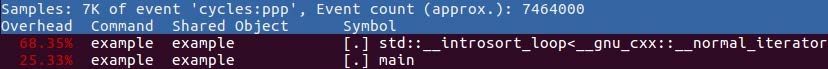
\includegraphics[width=0.9\textwidth]{content/1/chapter2/images/29.jpg}\\
图 2.29
\end{center}

The initial version of the code used the unsigned int index and a boundary condition in the loop (the last line); simply dropping that boundary condition check as entirely unnecessary results in a surprising performance degradation (the middle line); finally, changing the index to a signed int recovers the lost performance and even improves it (the first line).

Compiling the code fragments separately is usually enough to avoid any unwanted optimizations. Less commonly, you may find that the compiler does different optimizations to a particular chunk of code depending on what else is in the same file. This could be simply a bug in the compiler, but it can also be a result of some heuristic that is, in the experience of the compiler writers, more often right than not. If you observe that the results depend on some code that is not executed at all, only compiled, this may be the reason. One solution is to use the compilation unit from the real program and just call the function that you want to benchmark. Of course, you will have to satisfy compilation and link dependencies, so here is yet another reason to write modular code and minimize dependencies.

The other source of the context is the state of the computer itself. Obviously, if the entire program ran out of memory and is cycling pages in and out of swap, your small memory benchmark will not be representative of the real problem; on the other hand, the problem now is not in the "slow" code, the problem is that too much memory is consumed elsewhere. However, more subtle versions of this context dependency exist and may affect the benchmarks. A tell-tale sign of this situation is usually this: the results depend on the order in which the tests are executed (in the micro-benchmark, it is the order of the BENCHMARK macros). If reordering the tests or running just a subset of tests gives different results, there is some sort of dependency between them. It could be a code dependency, often as straightforward as data accumulation in some global data structure. Or it could be a subtle dependency on the hardware state. Those are much harder to figure out, but you will learn about some situations that lead to such dependencies later in this book.

Finally, there is a major source of context dependency that is entirely in your hands (which does not necessarily make it easy to avoid, but at least possible). It is the dependency on the state of your program. We already had to deal with the most obvious aspect of such dependency: the inputs to the code we want to benchmark. Sometimes, the inputs are known or can be reconstructed. Often, the performance problem happens only for certain kinds of inputs, and we don't know what is so special about them until we analyze the performance of the code with these specific inputs, which is exactly what we were trying to do with the micro-benchmark in the first place. In such cases, it is often the easiest to capture the inputs from the real run of the real program, store them in a file, and use them to recreate the state of the code we're measuring. This input could be as simple as a collection of data or as complex as a sequence of events that need to be recorded and "played back" to an event handler to reproduce the desired behavior.

The more complex the state we need to reconstruct is, the harder it is to reproduce the performance behavior of the real program in a partial benchmark. Note that this problem somewhat resembles the problem of writing unit tests: they, too, are much harder to write if the program cannot be broken up into smaller units with a simpler state. Once again, we see the advantages of a well-designed software system: a codebase with good unit test coverage is usually much easier to micro-benchmark, piece by piece.

As you were warned when we started this section, it is meant to partially restore your faith in micro-benchmarks. They can be a useful tool, as we will see many times in this book. They can also lead you astray, sometimes very far. You now understand some of the reasons why and are better prepared to try to recover the useful bits of information from the results, rather than giving up on small-scale benchmarking altogether.

None of the tools we have presented in this chapter is a solution to every problem; they are not meant to be. You can achieve the best results by using these tools to collect information in various ways, so they complement each other.






